\documentclass[aspectratio=169,10pt]{beamer}
\usetheme{Madrid}
\usecolortheme{seahorse}
\usepackage{fontspec}
\setsansfont{Noto Sans}
\setmonofont{Noto Sans Mono}[Scale=0.86]
\usepackage{booktabs,tabularx,array,multicol}
\usepackage{tikz}
\usetikzlibrary{positioning,arrows.meta,shapes.geometric,calc}
\usepackage{listings}
\usepackage{xcolor}
\definecolor{NEUBlue}{HTML}{16436B}
\definecolor{NEUGreen}{HTML}{086E56}
\definecolor{NEUPale}{HTML}{EFF5FA}
\definecolor{SQLBlue}{HTML}{114EAA}
\definecolor{SQLGreen}{HTML}{08704D}
\definecolor{SQLGray}{HTML}{5B6574}
\definecolor{SQLBG}{HTML}{F7FAFD}
\definecolor{NEURed}{HTML}{A82F38}
\definecolor{NEUOrange}{HTML}{AA6500}
\setbeamercolor{structure}{fg=NEUBlue}
\setbeamercolor{frametitle}{fg=white,bg=NEUBlue}
\setbeamercolor{title}{fg=white,bg=NEUBlue}
\setbeamercolor{block title}{bg=NEUBlue,fg=white}
\setbeamercolor{block body}{bg=NEUPale,fg=black}
\setbeamercolor{alertblock title}{bg=NEURed,fg=white}
\setbeamercolor{alertblock body}{bg=red!5,fg=black}
\setbeamertemplate{navigation symbols}{}
\setbeamertemplate{footline}[frame number]
\setbeamertemplate{itemize items}[circle]
\setbeamertemplate{blocks}[rounded][shadow=false]
\setbeamersize{text margin left=0.8cm,text margin right=0.8cm}
\lstdefinelanguage{MySQL}{
morekeywords={SELECT,FROM,WHERE,AS,DISTINCT,ORDER,BY,ASC,DESC,LIMIT,OFFSET,AND,OR,NOT,LIKE,IN,BETWEEN,IS,NULL,JOIN,INNER,LEFT,RIGHT,CROSS,ON,COUNT,SUM,AVG,MIN,MAX,GROUP,HAVING,CASE,WHEN,THEN,ELSE,END,IF,IFNULL,COALESCE,NULLIF,CONCAT,USE,SHOW,TABLES,DESC,DESCRIBE,EXISTS,ANY,ALL,EXPLAIN,TRUE,FALSE},
sensitive=false,morecomment=[l]{--},morestring=[b]' }
\lstdefinestyle{sql}{language=MySQL,basicstyle=\ttfamily\footnotesize,keywordstyle=\color{SQLBlue}\bfseries,commentstyle=\color{SQLGray},stringstyle=\color{SQLGreen},backgroundcolor=\color{SQLBG},frame=single,rulecolor=\color{black!18},columns=fullflexible,keepspaces=true,breaklines=true,breakatwhitespace=true,showstringspaces=false,xleftmargin=.35em,xrightmargin=.35em,aboveskip=.5em,belowskip=.5em}
\lstset{style=sql}
\newcommand{\code}[1]{\texttt{#1}}
\newcommand{\kw}[1]{\textcolor{NEUBlue}{\bfseries #1}}
\newcommand{\sourceurl}{\url{https://vudmvn.github.io/dbms-course/lectures/MySQL/querying-data/select/select-statement-5/}}
\title[SQL SELECT 5]{SELECT 5: Truy vấn con (Subqueries) trong MySQL}
\subtitle{Khái niệm -- Cú pháp -- Giải thích -- Ví dụ -- Bài tập}
\author{DBMS Course}
\institute{Smart Logistics and Supply Chain Management Lab}
\date{2026}
\begin{document}
\begin{frame}[plain]\titlepage\end{frame}
\begin{frame}[fragile]{Mục tiêu học tập}
\begin{columns}[T,onlytextwidth]
\column{.49\textwidth}
\begin{block}{Nhận biết \& giải thích}
\begin{itemize}
\item Subquery là gì; xuất hiện ở những mệnh đề nào.
\item Phân biệt kết quả trả về một giá trị và nhiều dòng.
\item Hiểu truy vấn con \textbf{tương quan} và không tương quan.
\end{itemize}
\end{block}
\column{.49\textwidth}
\begin{block}{Viết và kiểm tra SQL}
\begin{itemize}
\item \code{IN}, \code{NOT IN}; \code{EXISTS}, \code{NOT EXISTS}.
\item Subquery trong \code{SELECT}, \code{FROM}.
\item Nhận diện lỗi \code{NULL}, sai số dòng và thiếu bí danh.
\end{itemize}
\end{block}
\end{columns}
\end{frame}

\begin{frame}[fragile]{Mạch kiến thức của SELECT 5}
\begin{center}
\begin{tikzpicture}[x=1cm,y=1cm, >=Latex, every node/.style={font=\small,align=center}]
\node[draw=NEUBlue,thick,rounded corners,fill=NEUPale,minimum width=3.2cm,minimum height=1.0cm] (a) at (2.0,2.0) {Scalar subquery\\1 giá trị};
\node[draw=NEUBlue,thick,rounded corners,fill=NEUPale,minimum width=3.2cm,minimum height=1.0cm] (b) at (6.3,2.0) {Subquery nhiều dòng\\\code{IN / NOT IN}};
\node[draw=NEUBlue,thick,rounded corners,fill=NEUPale,minimum width=3.2cm,minimum height=1.0cm] (c) at (10.6,2.0) {Kiểm tra tồn tại\\\code{EXISTS / NOT EXISTS}};
\node[draw=NEUGreen,thick,rounded corners,fill=green!6,minimum width=4.0cm,minimum height=1cm] (d) at (4.2,.15) {Correlated subquery\\tham chiếu dòng ngoài};
\node[draw=NEUGreen,thick,rounded corners,fill=green!6,minimum width=4.0cm,minimum height=1cm] (e) at (8.6,.15) {Derived table\\subquery trong \code{FROM}};
\draw[->,thick,NEUBlue] (a)--(b);\draw[->,thick,NEUBlue] (b)--(c);
\draw[->,thick,NEUGreen] (b.south) -- (d.north);
\draw[->,thick,NEUGreen] (c.south) -- (e.north);
\end{tikzpicture}
\end{center}
\vspace{.3em}
\small{Ngữ cảnh ví dụ: cơ sở dữ liệu \code{classicmodels}.}
\end{frame}

\begin{frame}[fragile]{Các bảng cần dùng trong classicmodels}
\begin{columns}[T,onlytextwidth]
\column{.49\textwidth}
\small
\begin{tabularx}{\linewidth}{>{\ttfamily}l X}\toprule
Bảng & Dữ liệu\\\midrule
customers & Khách hàng\\
orders & Đơn hàng\\
orderdetails & Chi tiết đơn\\
payments & Thanh toán\\\bottomrule
\end{tabularx}
\column{.49\textwidth}
\small
\begin{tabularx}{\linewidth}{>{\ttfamily}l X}\toprule
Bảng & Dữ liệu\\\midrule
products & Sản phẩm\\
productlines & Dòng sản phẩm\\
employees & Nhân viên\\
offices & Văn phòng\\\bottomrule
\end{tabularx}
\end{columns}
\vspace{.5em}
\small \textbf{Khóa liên kết:} \code{orders.customerNumber} $\rightarrow$ \code{customers.customerNumber}; \code{orderdetails.productCode} $\rightarrow$ \code{products.productCode}.
\end{frame}

\begin{frame}[fragile]{Quan hệ bảng phục vụ các truy vấn con}
\begin{center}
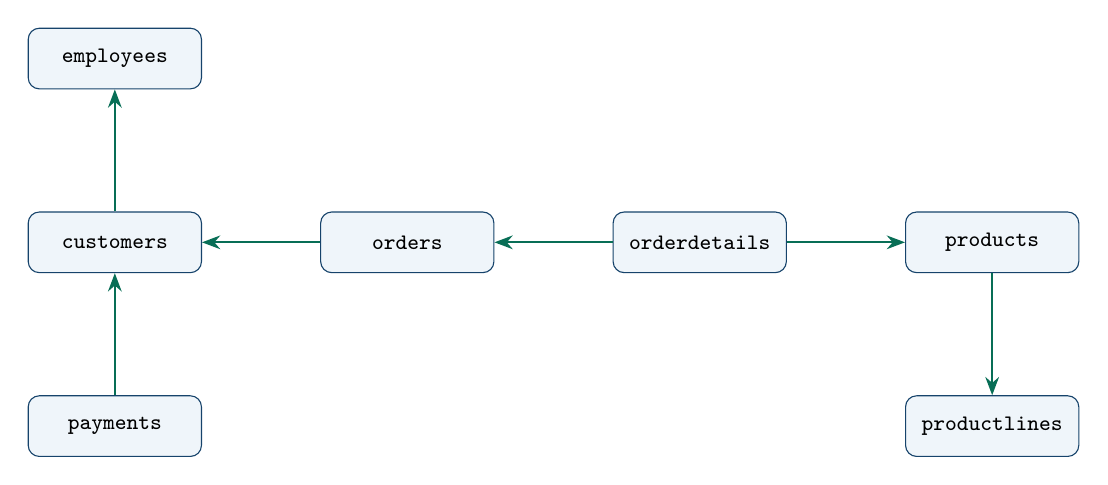
\begin{tikzpicture}[>=Stealth, node distance=1.55cm and 1.5cm,
 box/.style={draw=NEUBlue,rounded corners,fill=NEUPale,align=center,font=\footnotesize\ttfamily,minimum width=2.2cm,minimum height=.77cm}]
\node[box] (c) {customers};
\node[box,right=of c] (o) {orders};
\node[box,right=of o] (od) {orderdetails};
\node[box,right=of od] (p) {products};
\node[box,below=of c] (py) {payments};
\node[box,above=of c] (e) {employees};
\node[box,below=of p] (pl) {productlines};
\draw[->,thick,NEUGreen] (o)--(c);
\draw[->,thick,NEUGreen] (od)--(o);
\draw[->,thick,NEUGreen] (od)--(p);
\draw[->,thick,NEUGreen] (py)--(c);
\draw[->,thick,NEUGreen] (c)--(e);
\draw[->,thick,NEUGreen] (p)--(pl);
\end{tikzpicture}
\end{center}
\vspace{.1em}
\small Mũi tên cho biết bảng chứa khóa ngoại $\rightarrow$ bảng được tham chiếu; điều kiện so sánh trong SQL phải sử dụng đúng cặp khóa.
\end{frame}

\begin{frame}[fragile]{Khởi động MySQL và khám phá bảng}
\begin{lstlisting}
USE classicmodels;
SHOW TABLES;
DESC products;
DESC customers;
DESC orders;
DESC orderdetails;
\end{lstlisting}
\begin{itemize}
\item \code{USE}: chọn CSDL đang làm việc.
\item \code{SHOW TABLES}: liệt kê bảng.
\item \code{DESC}: xem cột, kiểu dữ liệu và khóa.
\end{itemize}
\end{frame}

\section{Khái niệm truy vấn con}

\begin{frame}[fragile]{Subquery là gì?}
\begin{block}{Định nghĩa}
Truy vấn con (\emph{subquery}) là một câu lệnh \code{SELECT} nằm trong câu truy vấn khác.
\end{block}
\begin{lstlisting}
SELECT productCode, productName, buyPrice
FROM products
WHERE buyPrice > (
    SELECT AVG(buyPrice)
    FROM products
);
\end{lstlisting}
\begin{enumerate}
\item \textbf{Truy vấn trong:} tính giá mua trung bình.
\item \textbf{Truy vấn ngoài:} giữ những sản phẩm có giá lớn hơn ngưỡng đó.
\end{enumerate}
\end{frame}

\begin{frame}[fragile]{Cách đọc truy vấn con theo hai tầng}
\begin{center}
\begin{tikzpicture}[x=1cm,y=1cm,>=Stealth]
\node[draw=NEUBlue,thick,rounded corners,fill=NEUPale,text width=3.8cm,align=center,minimum height=1.4cm] (inner) at (2.4,1.5) {\textbf{Inner query}\\\code{AVG(buyPrice)}\\trả một con số};
\node[draw=NEUGreen,thick,rounded corners,fill=green!7,text width=4.5cm,align=center,minimum height=1.4cm] (outer) at (9.0,1.5) {\textbf{Outer query}\\\code{WHERE buyPrice > ...}\\lọc các sản phẩm};
\draw[->,line width=1.4pt,NEUBlue] (inner)--node[above,font=\small]{Giá trị ngưỡng} (outer);
\end{tikzpicture}
\end{center}
\begin{alertblock}{Chú ý về thực thi}
Đây là \textbf{cách hiểu logic}, không nhất thiết là kế hoạch thực thi vật lý: MySQL có thể tối ưu hóa hoặc viết lại truy vấn.
\end{alertblock}
\end{frame}

\begin{frame}[fragile]{Subquery có thể xuất hiện ở đâu?}
\small
\begin{tabularx}{\linewidth}{>{\ttfamily}l X X}\toprule
Vị trí & Vai trò & Ví dụ sử dụng\\\midrule
WHERE & Lọc dòng theo kết quả của câu khác & So sánh với AVG; IN / EXISTS\\
SELECT & Sinh thêm giá trị / cột & Đếm đơn hàng mỗi khách\\
FROM & Tạo derived table & Tổng doanh thu theo đơn\\
HAVING & Lọc nhóm bằng điều kiện con & So với trung bình các nhóm\\\bottomrule
\end{tabularx}
\vspace{.7em}
\begin{block}{Ghi nhớ}
\small Kết quả của subquery có thể là \textbf{1 giá trị}, \textbf{nhiều dòng (1 cột)}, hoặc \textbf{một bảng nhiều cột}. Toán tử bên ngoài phải phù hợp với hình dạng kết quả.
\end{block}
\end{frame}

\begin{frame}[fragile]{Phân loại theo dạng kết quả và quan hệ}
\small
\begin{tabularx}{\linewidth}{l X}\toprule
Tiêu chí & Các trường hợp\\\midrule
Số giá trị & Scalar (một giá trị); một cột nhiều dòng; bảng nhiều cột\\
Phụ thuộc & Non-correlated (độc lập); correlated (tham chiếu truy vấn ngoài)\\
Mục đích & So sánh; thành viên tập hợp; tồn tại; tạo cột; tạo bảng nguồn\\\bottomrule
\end{tabularx}
\vspace{.6em}
\begin{alertblock}{Lưu ý}
\small Không thể tùy ý dùng \code{=} với subquery có nhiều dòng. Trong MySQL, scalar subquery nhiều dòng sẽ phát sinh lỗi \emph{Subquery returns more than 1 row}.
\end{alertblock}
\end{frame}

\section{Scalar subquery}

\begin{frame}[fragile]{Scalar subquery: cú pháp và thành phần}
\begin{lstlisting}
SELECT column_list
FROM table_name
WHERE value_expression > (
    SELECT aggregate_function(column)
    FROM another_table
);
\end{lstlisting}
\begin{block}{Giải thích cú pháp}
\begin{itemize}
\item \code{(SELECT ...)}: câu truy vấn con trả về tối đa một dòng, một cột.
\item \code{value\_expression}: giá trị của dòng đang xét.
\item \code{>}: toán tử so sánh, có thể thay bằng \code{=}, \code{<>}, \code{<}, \code{<=}, \code{>=}.
\end{itemize}
\end{block}
\end{frame}

\begin{frame}[fragile]{Ví dụ: giá mua cao hơn trung bình}
\begin{lstlisting}
SELECT productCode, productName, buyPrice
FROM products
WHERE buyPrice > (
    SELECT AVG(buyPrice)
    FROM products
);
\end{lstlisting}
\begin{columns}[T,onlytextwidth]
\column{.49\textwidth}
\begin{block}{Subquery}
\code{AVG(buyPrice)} trả về một con số đại diện cho toàn bộ bảng.
\end{block}
\column{.49\textwidth}
\begin{block}{Outer query}
Kiểm tra \code{buyPrice > trung bình} trên từng sản phẩm.
\end{block}
\end{columns}
\small Đầu ra: các sản phẩm đắt hơn mức giá mua trung bình (không gồm bằng ngưỡng).
\end{frame}

\begin{frame}[fragile]{Bước tính scalar subquery: ví dụ số}
\small \textbf{Dữ liệu giả lập để minh họa} (không phải dữ liệu thật của classicmodels):
\begin{center}
\begin{tabular}{lrr}\toprule
Sản phẩm & buyPrice & So với trung bình?\\\midrule
P1 & 30 & Không\\
P2 & 50 & Không\\
P3 & 70 & Có\\
P4 & 90 & Có\\\bottomrule
\end{tabular}
\end{center}
\[\mathrm{AVG}=(30+50+70+90)/4=60\]
\begin{block}{Ghi nhớ}
\small Truy vấn ngoài chỉ giữ P3 và P4, vì 70 và 90 lớn hơn 60.
\end{block}
\end{frame}

\begin{frame}[fragile]{Ví dụ: tìm sản phẩm có MSRP cao nhất}
\begin{lstlisting}
SELECT productCode, productName, MSRP
FROM products
WHERE MSRP = (
    SELECT MAX(MSRP)
    FROM products
);
\end{lstlisting}
\begin{itemize}
\item Subquery trả \textbf{giá MSRP lớn nhất}.
\item \code{=} giữ tất cả sản phẩm có đúng MSRP đó.
\item Nếu nhiều sản phẩm cùng có MSRP tối đa, câu lệnh trả về \textbf{nhiều dòng} (hoàn toàn hợp lệ).
\end{itemize}
\end{frame}

\begin{frame}[fragile]{Ví dụ: khoản thanh toán lớn hơn trung bình}
\begin{lstlisting}
SELECT customerNumber, checkNumber,
       paymentDate, amount
FROM payments
WHERE amount > (
    SELECT AVG(amount)
    FROM payments
);
\end{lstlisting}
\begin{block}{Ý nghĩa}
Đưa ra các khoản thanh toán vượt mức trung bình. Khác với truy vấn trên \code{products}, nguồn dữ liệu được thay thành \code{payments}.
\end{block}
\end{frame}

\begin{frame}[fragile]{Bẫy: scalar subquery nhiều hơn một dòng}
\textbf{Viết sai:}\begin{lstlisting}
SELECT customerNumber, customerName
FROM customers
WHERE customerNumber = (
    SELECT customerNumber
    FROM orders
);
\end{lstlisting}
\begin{alertblock}{Lưu ý}
\small Truy vấn con có thể trả về nhiều mã khách hàng; trong MySQL, dùng \code{=} như vậy sẽ lỗi (trừ khi thực tế chỉ có tối đa 1 dòng).
\end{alertblock}
\small \textbf{Cách sửa:} khi mục tiêu là thuộc tập giá trị, dùng \code{IN} hoặc \code{EXISTS}.
\end{frame}

\section{IN / NOT IN}

\begin{frame}[fragile]{IN với subquery: cú pháp}
\begin{lstlisting}
SELECT column_list
FROM outer_table
WHERE key_column IN (
    SELECT matching_key
    FROM inner_table
);
\end{lstlisting}
\begin{block}{Giải thích cú pháp}
\begin{itemize}
\item Subquery phải trả về \textbf{một cột} để so khớp với một khóa.
\item \code{IN} kiểm tra giá trị của dòng ngoài có thuộc tập con hay không.
\item Các giá trị lặp trong tập con không làm dòng ngoài bị nhân bản.
\end{itemize}
\end{block}
\end{frame}

\begin{frame}[fragile]{IN: khách hàng đã từng đặt hàng}
\begin{lstlisting}
SELECT customerNumber, customerName
FROM customers
WHERE customerNumber IN (
    SELECT customerNumber
    FROM orders
);
\end{lstlisting}
\begin{itemize}
\item \code{orders} cung cấp tập mã khách hàng có đơn hàng.
\item \code{customers} cung cấp thông tin tên khách hàng.
\item Mỗi khách hàng được trả \textbf{tối đa một lần} nếu bảng customers có khóa chính duy nhất.
\end{itemize}
\end{frame}

\begin{frame}[fragile]{IN: sản phẩm đã từng được đặt}
\begin{lstlisting}
SELECT productCode, productName
FROM products
WHERE productCode IN (
    SELECT productCode
    FROM orderdetails
);
\end{lstlisting}
\begin{block}{Ghi nhớ}
\small Đây là truy vấn kiểu \emph{membership}: một sản phẩm có thể nằm ở 100 dòng orderdetails nhưng vẫn chỉ xuất hiện một lần trong kết quả từ products.
\end{block}
\end{frame}

\begin{frame}[fragile]{IN và JOIN: có thể khác số dòng}
\small
\begin{columns}[T,onlytextwidth]
\column{.48\textwidth}
\begin{block}{IN}
\code{products} là nguồn của kết quả. Mỗi sản phẩm phù hợp chỉ xuất hiện một lần (nếu khóa duy nhất).
\end{block}
\column{.48\textwidth}
\begin{block}{INNER JOIN}
Nếu nối trực tiếp \code{products} với \code{orderdetails}, một sản phẩm có thể lặp lại cho từng dòng chi tiết.
\end{block}
\end{columns}
\vspace{.5em}
\begin{alertblock}{Lưu ý}
\small Nếu mục tiêu là \textbf{tồn tại ít nhất một} đơn hàng, dùng \code{IN} hoặc \code{EXISTS} có thể biểu đạt ý định rõ hơn JOIN trực tiếp.
\end{alertblock}
\end{frame}

\begin{frame}[fragile]{NOT IN: cú pháp và ý nghĩa}
\begin{lstlisting}
SELECT column_list
FROM outer_table
WHERE key_column NOT IN (
    SELECT matching_key
    FROM inner_table
);
\end{lstlisting}
\begin{block}{Giải thích}
\begin{itemize}
\item \code{NOT IN} chọn các giá trị \textbf{không thuộc} tập subquery.
\item Hữu ích để tìm khách hàng chưa đặt, sản phẩm chưa được mua.
\item Chỉ an toàn khi hiểu rõ khả năng xuất hiện \code{NULL} trong subquery.
\end{itemize}
\end{block}
\end{frame}

\begin{frame}[fragile]{NOT IN: sản phẩm chưa từng được đặt}
\begin{lstlisting}
SELECT productCode, productName
FROM products
WHERE productCode NOT IN (
    SELECT productCode
    FROM orderdetails
);
\end{lstlisting}
\begin{itemize}
\item Subquery: các mã sản phẩm đã được đặt.
\item Truy vấn ngoài: sản phẩm không nằm trong tập này.
\item Nếu \code{orderdetails.productCode} không \code{NULL}, cách viết này dễ hiểu.
\end{itemize}
\end{frame}

\begin{frame}[fragile]{Bẫy 3 giá trị: NOT IN và NULL}
\small Giả sử truy vấn con trả về tập \code{(10, 20, NULL)}.
\begin{center}
\begin{tabular}{l c l}\toprule
Điều kiện & SQL logic & Có vào kết quả?\\\midrule
\code{10 NOT IN (10,20,NULL)} & FALSE & Không\\
\code{30 NOT IN (10,20,NULL)} & UNKNOWN & Không\\
\code{30 NOT IN (10,20)} & TRUE & Có\\\bottomrule
\end{tabular}
\end{center}
\begin{alertblock}{Lưu ý}
\small Mệnh đề \code{WHERE} chỉ giữ giá trị \code{TRUE}; \code{FALSE} và \code{UNKNOWN} đều bị loại. \code{NOT IN} với \code{NULL} có thể làm kết quả bất ngờ rỗng.
\end{alertblock}
\end{frame}

\begin{frame}[fragile]{Cách sửa NOT IN: loại NULL ở truy vấn con}
\begin{lstlisting}
SELECT employeeNumber, lastName, firstName
FROM employees
WHERE employeeNumber NOT IN (
    SELECT salesRepEmployeeNumber
    FROM customers
    WHERE salesRepEmployeeNumber IS NOT NULL
);
\end{lstlisting}
\begin{block}{Ghi nhớ}
\small Bộ lọc \code{IS NOT NULL} ngăn giá trị NULL của nhân viên phụ trách làm sai nghĩa phép \code{NOT IN}.
\end{block}
\end{frame}

\begin{frame}[fragile]{Giải pháp thay thế: NOT EXISTS}
\begin{lstlisting}
SELECT e.employeeNumber, e.lastName, e.firstName
FROM employees AS e
WHERE NOT EXISTS (
    SELECT 1
    FROM customers AS c
    WHERE c.salesRepEmployeeNumber = e.employeeNumber
);
\end{lstlisting}
\begin{itemize}
\item Kiểm tra không có khách hàng nào liên kết với nhân viên đang xét.
\item Không bị bẫy \code{NULL} ở bảng trong theo cách \code{NOT IN} gặp phải.
\end{itemize}
\end{frame}

\section{Subquery trong SELECT}

\begin{frame}[fragile]{Subquery trong SELECT: cú pháp}
\begin{lstlisting}
SELECT o.key_column,
       o.descriptive_column,
       (
           SELECT COUNT(*)
           FROM inner_table AS i
           WHERE i.foreign_key = o.key_column
       ) AS relatedCount
FROM outer_table AS o;
\end{lstlisting}
\begin{block}{Giải thích}
\begin{itemize}
\item Mỗi dòng ngoài có thêm một \textbf{cột tính toán}.
\item Subquery ở đây phải trả về \textbf{một giá trị} cho từng dòng ngoài.
\item Đặt \code{AS relatedCount} để cột mới có tên dễ hiểu.
\end{itemize}
\end{block}
\end{frame}

\begin{frame}[fragile]{Ví dụ: số đơn hàng của mỗi khách hàng}
\begin{lstlisting}
SELECT c.customerNumber, c.customerName,
       (
           SELECT COUNT(*)
           FROM orders AS o
           WHERE o.customerNumber = c.customerNumber
       ) AS orderCount
FROM customers AS c;
\end{lstlisting}
\begin{itemize}
\item Vế \code{o.customerNumber = c.customerNumber} tạo sự liên kết với dòng ngoài.
\item \code{COUNT(*)} bằng 0 nếu khách hàng không có đơn nào.
\item Kết quả vẫn có \textbf{mọi khách hàng} trong bảng ngoài.
\end{itemize}
\end{frame}

\begin{frame}[fragile]{Ví dụ: tổng thanh toán của mỗi khách hàng}
\begin{lstlisting}
SELECT c.customerNumber, c.customerName,
       (
           SELECT SUM(p.amount)
           FROM payments AS p
           WHERE p.customerNumber = c.customerNumber
       ) AS totalPayment
FROM customers AS c;
\end{lstlisting}
\begin{alertblock}{Lưu ý}
\small Với khách hàng không có khoản thanh toán, \code{SUM} trả \code{NULL}, không phải 0. Có thể dùng \code{COALESCE(..., 0)} nếu muốn hiển thị 0.
\end{alertblock}
\end{frame}

\begin{frame}[fragile]{COALESCE: thay NULL bằng 0 khi tính tổng}
\begin{lstlisting}
SELECT c.customerNumber, c.customerName,
       COALESCE((
           SELECT SUM(p.amount)
           FROM payments AS p
           WHERE p.customerNumber = c.customerNumber
       ), 0) AS totalPayment
FROM customers AS c;
\end{lstlisting}
\begin{block}{Ghi nhớ}
\small \code{COALESCE(expression, 0)} lấy \code{expression} nếu khác NULL; ngược lại trả 0.
\end{block}
\end{frame}

\begin{frame}[fragile]{Subquery trong SELECT: những điều cần nhớ}
\begin{itemize}
\item Subquery có thể sử dụng \code{COUNT}, \code{SUM}, \code{AVG} hoặc truy vấn một giá trị.
\item Nếu truy vấn con trả nhiều dòng thì không dùng trực tiếp làm một ô dữ liệu.
\item Subquery tương quan có thể đọc rõ hơn trong những bài toán \emph{đếm / tính tổng theo từng đối tượng}.
\item Với báo cáo dữ liệu lớn, có thể cân nhắc \code{JOIN + GROUP BY} hoặc bảng tổng hợp.
\end{itemize}
\end{frame}

\section{Correlated subquery}

\begin{frame}[fragile]{Correlated subquery là gì?}
\begin{block}{Định nghĩa}
\textbf{Correlated subquery} tham chiếu cột hoặc bí danh của truy vấn ngoài, ví dụ \code{p.productLine} trong điều kiện của truy vấn con.
\end{block}
\begin{lstlisting}
SELECT p.productCode, p.productName
FROM products AS p
WHERE p.buyPrice > (
    SELECT AVG(p2.buyPrice)
    FROM products AS p2
    WHERE p2.productLine = p.productLine
);
\end{lstlisting}
\begin{block}{Ghi nhớ}
\small Ngưỡng so sánh thay đổi theo \textbf{dòng sản phẩm} của mỗi \code{p}.
\end{block}
\end{frame}

\begin{frame}[fragile]{Non-correlated và correlated: so sánh}
\small
\begin{tabularx}{\linewidth}{l X X}\toprule
 & Không tương quan & Tương quan\\\midrule
Tham chiếu & Chỉ cột của truy vấn con & Có cột của truy vấn ngoài\\
Ngưỡng & Có thể chung cho tất cả dòng & Có thể khác theo từng dòng\\
Ví dụ & So với AVG toàn bộ sản phẩm & So với AVG cùng productLine\\\bottomrule
\end{tabularx}
\vspace{.7em}
\begin{alertblock}{Lưu ý}
\small Đừng đồng nhất cách hiểu \emph{``theo từng dòng} với việc DBMS chắc chắn chạy riêng subquery cho từng dòng. Bộ tối ưu MySQL có thể biến đổi cách thực thi.
\end{alertblock}
\end{frame}

\begin{frame}[fragile]{Vì sao điều kiện tương quan rất quan trọng?}
\begin{lstlisting}
SELECT p.productCode, p.productName, p.productLine
FROM products AS p
WHERE p.MSRP > (
    SELECT AVG(p2.MSRP)
    FROM products AS p2
    WHERE p2.productLine = p.productLine
);
\end{lstlisting}
\begin{itemize}
\item Bỏ dòng \code{p2.productLine = p.productLine}: trở thành so với trung bình toàn bộ sản phẩm.
\item Giữ dòng đó: so với trung bình \textbf{cùng dòng sản phẩm}.
\item Hai câu hỏi kinh doanh khác nhau, có thể cho kết quả rất khác.
\end{itemize}
\end{frame}

\begin{frame}[fragile]{Minh họa nhóm: ngưỡng thay đổi theo từng dòng}
\small \textbf{Dữ liệu giả lập:}
\begin{center}
\begin{tabular}{l c r r c}\toprule
Sản phẩm & Line & Giá & Trung bình line & Đạt?\\\midrule
P1 & Classic & 100 & 75 & Có\\
P2 & Classic & 50 & 75 & Không\\
P3 & Motorcycle & 30 & 40 & Không\\
P4 & Motorcycle & 50 & 40 & Có\\\bottomrule
\end{tabular}
\end{center}
\vspace{.2em}
\begin{block}{Ghi nhớ}
\small Cùng một biểu thức \code{AVG}, nhưng nhóm so sánh của P1 và P3 khác nhau.
\end{block}
\end{frame}

\begin{frame}[fragile]{Correlated COUNT: khách hàng có hơn 3 đơn}
\begin{lstlisting}
SELECT c.customerNumber, c.customerName
FROM customers AS c
WHERE (
    SELECT COUNT(*)
    FROM orders AS o
    WHERE o.customerNumber = c.customerNumber
) > 3;
\end{lstlisting}
\begin{block}{Cách đọc}
\begin{itemize}
\item Với từng khách hàng \code{c}, tính số đơn mang cùng \code{customerNumber}.
\item Chỉ giữ khách hàng có \code{orderCount > 3}.
\end{itemize}
\end{block}
\end{frame}

\section{EXISTS / NOT EXISTS}

\begin{frame}[fragile]{EXISTS: cú pháp và giải thích}
\begin{lstlisting}
SELECT o.column_list
FROM outer_table AS o
WHERE EXISTS (
    SELECT 1
    FROM inner_table AS i
    WHERE i.foreign_key = o.primary_key
);
\end{lstlisting}
\begin{itemize}
\item \code{EXISTS} cho \code{TRUE} khi subquery có ít nhất một dòng.
\item \code{SELECT 1} là quy ước dễ đọc; nội dung biểu thức trong SELECT không quyết định điều kiện tồn tại.
\item Phù hợp với câu hỏi \emph{có ít nhất một ...?}.
\end{itemize}
\end{frame}

\begin{frame}[fragile]{EXISTS: khách hàng đã từng đặt hàng}
\begin{lstlisting}
SELECT c.customerNumber, c.customerName
FROM customers AS c
WHERE EXISTS (
    SELECT 1
    FROM orders AS o
    WHERE o.customerNumber = c.customerNumber
);
\end{lstlisting}
\begin{block}{Giải thích}
\begin{itemize}
\item Một khách hàng được giữ khi có ít nhất một đơn hàng liên quan.
\item Không cần đếm tổng số đơn nếu chỉ kiểm tra sự tồn tại.
\end{itemize}
\end{block}
\end{frame}

\begin{frame}[fragile]{EXISTS: sản phẩm có đơn hàng}
\begin{lstlisting}
SELECT p.productCode, p.productName
FROM products AS p
WHERE EXISTS (
    SELECT 1
    FROM orderdetails AS od
    WHERE od.productCode = p.productCode
);
\end{lstlisting}
\begin{block}{Ghi nhớ}
\small Kết quả giống ý định của \code{IN}, nhưng \code{EXISTS} biểu diễn trực tiếp câu hỏi có ít nhất một dòng chi tiết không.
\end{block}
\end{frame}

\begin{frame}[fragile]{EXISTS: mô phỏng từng dòng ngoài}
\small\textbf{Ví dụ giả lập:}\vspace{.3em}
\begin{center}
\begin{tabular}{lcc}\toprule
Khách hàng & Số đơn tìm được & EXISTS?\\\midrule
C101 & 3 & TRUE\\
C102 & 0 & FALSE\\
C103 & 1 & TRUE\\\bottomrule
\end{tabular}
\end{center}
\vspace{.3em}
\begin{columns}[T,onlytextwidth]
\column{.49\textwidth}
\begin{block}{EXISTS}
Giữ \code{C101} và \code{C103}.
\end{block}
\column{.49\textwidth}
\begin{block}{NOT EXISTS}
Chỉ giữ \code{C102}.
\end{block}
\end{columns}
\end{frame}

\begin{frame}[fragile]{NOT EXISTS: cú pháp}
\begin{lstlisting}
SELECT o.column_list
FROM outer_table AS o
WHERE NOT EXISTS (
    SELECT 1
    FROM inner_table AS i
    WHERE i.foreign_key = o.primary_key
);
\end{lstlisting}
\begin{itemize}
\item Trả về các dòng \emph{không có} bản ghi phù hợp ở bảng liên quan.
\item Khác với \code{NOT IN}, cách kiểm tra sự tồn tại không bị ảnh hưởng bởi NULL trong các giá trị không liên quan.
\end{itemize}
\end{frame}

\begin{frame}[fragile]{NOT EXISTS: khách hàng chưa có đơn hàng}
\begin{lstlisting}
SELECT c.customerNumber, c.customerName
FROM customers AS c
WHERE NOT EXISTS (
    SELECT 1
    FROM orders AS o
    WHERE o.customerNumber = c.customerNumber
);
\end{lstlisting}
\begin{block}{Ghi nhớ}
\small Trong điều kiện so sánh, \code{o.customerNumber = c.customerNumber} là liên kết quan trọng nhất: bỏ nó sẽ kiểm tra xem \emph{bất kỳ đơn hàng nào} tồn tại, không phải đơn của khách hiện tại.
\end{block}
\end{frame}

\begin{frame}[fragile]{NOT EXISTS: sản phẩm chưa từng được đặt}
\begin{lstlisting}
SELECT p.productCode, p.productName
FROM products AS p
WHERE NOT EXISTS (
    SELECT 1
    FROM orderdetails AS od
    WHERE od.productCode = p.productCode
);
\end{lstlisting}
\begin{itemize}
\item Phù hợp để phát hiện sản phẩm không xuất hiện trong chi tiết đơn.
\item Kỹ thuật này còn gọi là kiểm tra \emph{anti-existence}.
\end{itemize}
\end{frame}

\begin{frame}[fragile]{IN vs EXISTS vs NOT EXISTS: chọn kỹ thuật}
\small
\begin{tabularx}{\linewidth}{l X X}\toprule
Kỹ thuật & Câu hỏi điển hình & Lưu ý\\\midrule
\code{IN} & Khóa này có trong tập con? & Hợp với 1 cột nhiều dòng\\
\code{EXISTS} & Có ít nhất một dòng liên quan? & Thường là subquery tương quan\\
\code{NOT IN} & Khóa không thuộc tập con? & Cẩn thận NULL\\
\code{NOT EXISTS} & Không có dòng liên quan? & Ít rủi ro bẫy NULL\\\bottomrule
\end{tabularx}
\vspace{.6em}
\begin{block}{Ghi nhớ}
\small Tính hiệu quả phụ thuộc dữ liệu, chỉ mục và phiên bản MySQL; không khẳng định phương pháp nào luôn nhanh nhất.
\end{block}
\end{frame}

\section{Derived table}

\begin{frame}[fragile]{Derived table: cú pháp và vai trò}
\begin{lstlisting}
SELECT dt.column1, dt.aggregated_value
FROM (
    SELECT grouping_key AS column1,
           SUM(amount) AS aggregated_value
    FROM source_table
    GROUP BY grouping_key
) AS dt
WHERE dt.aggregated_value > threshold;
\end{lstlisting}
\begin{block}{Giải thích}
\begin{itemize}
\item Subquery trong \code{FROM} tạo một \textbf{quan hệ trung gian} nhiều dòng/cột.
\item \code{AS dt} đặt bí danh; trong MySQL derived table cần có bí danh.
\item Truy vấn ngoài tiếp tục lọc, sắp xếp hoặc nối dữ liệu của bảng trung gian.
\end{itemize}
\end{block}
\end{frame}

\begin{frame}[fragile]{Derived table: tổng thanh toán theo khách hàng}
\begin{lstlisting}
SELECT customerNumber, totalPayment
FROM (
    SELECT customerNumber,
           SUM(amount) AS totalPayment
    FROM payments
    GROUP BY customerNumber
) AS payment_summary
WHERE totalPayment > 100000;
\end{lstlisting}
\begin{enumerate}
\item Truy vấn trong gom \code{payments} theo \code{customerNumber}.
\item Tính \code{totalPayment} cho từng khách hàng.
\item Truy vấn ngoài giữ nhóm có tổng vượt 100000.
\end{enumerate}
\end{frame}

\begin{frame}[fragile]{Derived table: diễn giải bảng trung gian}
\small \textbf{Bảng tạm giả lập do subquery tạo ra:}
\begin{center}
\begin{tabular}{lr}\toprule
customerNumber & totalPayment\\\midrule
101 & 80,000\\
102 & 150,000\\
103 & 120,000\\
104 & 20,000\\\bottomrule
\end{tabular}
\end{center}
\vspace{.1em}
\begin{columns}[T,onlytextwidth]
\column{.49\textwidth}
\begin{block}{Subquery}
Tính \code{SUM(amount)} theo mã khách.
\end{block}
\column{.49\textwidth}
\begin{block}{Outer query}
Giữ khách \code{102} và \code{103} (tổng $>100000$).
\end{block}
\end{columns}
\end{frame}

\begin{frame}[fragile]{Derived table: doanh thu từng đơn hàng}
\begin{lstlisting}
SELECT orderNumber, orderTotal
FROM (
    SELECT orderNumber,
           SUM(quantityOrdered * priceEach)
               AS orderTotal
    FROM orderdetails
    GROUP BY orderNumber
) AS order_summary
WHERE orderTotal > 50000;
\end{lstlisting}
\begin{block}{Ghi nhớ}
\small Doanh thu từng đơn dùng \code{SUM(quantityOrdered * priceEach)}; không nhầm với số tiền \code{payments.amount}.
\end{block}
\end{frame}

\begin{frame}[fragile]{Derived table và HAVING: so sánh}
\begin{columns}[T,onlytextwidth]
\column{.48\textwidth}
\begin{block}{HAVING trực tiếp}
\begin{lstlisting}
SELECT customerNumber,
       SUM(amount) AS totalPayment
FROM payments
GROUP BY customerNumber
HAVING SUM(amount) > 100000;
\end{lstlisting}
\end{block}
\column{.48\textwidth}
\begin{block}{Derived table}
\begin{lstlisting}
SELECT customerNumber, totalPayment
FROM (
  SELECT customerNumber,
         SUM(amount) AS totalPayment
  FROM payments
  GROUP BY customerNumber
) AS t
WHERE totalPayment > 100000;
\end{lstlisting}
\end{block}
\end{columns}
\vspace{.2em}\footnotesize Hai cách thể hiện cùng mục tiêu trên cùng nguồn dữ liệu, nhưng derived table thuận tiện nếu cần nối/biến đổi kết quả đã tổng hợp.
\end{frame}

\begin{frame}[fragile]{Bí danh derived table và phạm vi của cột}
\textbf{Thiếu alias:}\begin{lstlisting}
SELECT *
FROM (
    SELECT customerNumber, SUM(amount) AS totalPayment
    FROM payments
    GROUP BY customerNumber
);
\end{lstlisting}
\textbf{Sửa lại:}\begin{lstlisting}
SELECT *
FROM (
    SELECT customerNumber, SUM(amount) AS totalPayment
    FROM payments
    GROUP BY customerNumber
) AS payment_summary;
\end{lstlisting}
\begin{block}{Ghi nhớ}
\small Derived table cần bí danh; chỉ những cột được \code{SELECT} bên trong mới dùng được ở ngoài.
\end{block}
\end{frame}

\section{Lỗi thường gặp và hiệu năng}

\begin{frame}[fragile]{Các lỗi subquery sinh viên thường mắc}
\small
\begin{tabularx}{\linewidth}{l X}\toprule
Lỗi & Cách kiểm tra / sửa\\\midrule
\code{=} với nhiều dòng & Dùng \code{IN} hoặc giới hạn về một giá trị\\
\code{NOT IN} có NULL & Lọc NULL hoặc thay bằng \code{NOT EXISTS}\\
Thiếu liên kết correlated & Kiểm tra điều kiện bằng khóa hai bảng\\
Thiếu alias derived table & Thêm \code{AS tên\_bảng\_tạm}\\
\code{SUM()} kỳ vọng 0 & Dùng \code{COALESCE(SUM(...),0)}\\
Lọc nhầm nhóm & Phân biệt \code{WHERE} và \code{HAVING}\\\bottomrule
\end{tabularx}
\end{frame}

\begin{frame}[fragile]{Lỗi correlated: quên điều kiện liên kết}
\textbf{Truy vấn có lỗi logic:}\begin{lstlisting}
SELECT c.customerNumber, c.customerName
FROM customers AS c
WHERE EXISTS (
    SELECT 1
    FROM orders AS o
);
\end{lstlisting}
\begin{alertblock}{Lưu ý}
\small Nếu bảng orders có bất kỳ dòng nào, EXISTS sẽ đúng với mọi khách hàng; không phải ``khách hàng đã đặt hàng.
\end{alertblock}
\textbf{Sửa: thêm} \code{WHERE o.customerNumber = c.customerNumber} \textbf{ở subquery}.
\end{frame}

\begin{frame}[fragile]{Tư duy hiệu năng: subquery và chỉ mục}
\begin{lstlisting}
EXPLAIN
SELECT c.customerNumber, c.customerName
FROM customers AS c
WHERE EXISTS (
    SELECT 1
    FROM orders AS o
    WHERE o.customerNumber = c.customerNumber
);
\end{lstlisting}
\begin{itemize}
\item Chỉ mục trên khóa liên kết (ví dụ \code{orders.customerNumber}) thường hữu ích.
\item Dùng \code{EXPLAIN} để xem kế hoạch thực thi thực tế.
\item MySQL có thể biến đổi \code{IN}/\code{EXISTS} thành chiến lược semi-join, tùy truy vấn và phiên bản.
\end{itemize}
\end{frame}

\section{Luyện tập có hướng dẫn}

\begin{frame}[fragile]{Luyện tập 1: scalar subquery (Bài 5.1)}
\textbf{Yêu cầu:} Sản phẩm có MSRP lớn hơn MSRP trung bình.\vspace{.2em}\begin{lstlisting}
SELECT productCode, productName, MSRP
FROM products
WHERE MSRP > (
    SELECT AVG(MSRP)
    FROM products
);
\end{lstlisting}
\begin{block}{Câu hỏi trên lớp}
Nếu một sản phẩm có \code{MSRP} đúng bằng trung bình, sản phẩm đó có được giữ lại không?
\end{block}
\end{frame}

\begin{frame}[fragile]{Luyện tập 2: IN (Bài 6.1)}
\textbf{Yêu cầu:} Liệt kê khách hàng đã từng có đơn hàng.\vspace{.2em}\begin{lstlisting}
SELECT customerNumber, customerName
FROM customers
WHERE customerNumber IN (
    SELECT customerNumber
    FROM orders
);
\end{lstlisting}
\begin{block}{Ghi nhớ}
\small Viết thêm một phiên bản sử dụng \code{EXISTS}, sau đó so sánh kết quả.
\end{block}
\end{frame}

\begin{frame}[fragile]{Luyện tập 3: NOT IN (Bài 7.4)}
\textbf{Yêu cầu:} Nhân viên chưa phụ trách khách hàng nào.\vspace{.2em}\begin{lstlisting}
SELECT employeeNumber, lastName, firstName
FROM employees
WHERE employeeNumber NOT IN (
    SELECT salesRepEmployeeNumber
    FROM customers
    WHERE salesRepEmployeeNumber IS NOT NULL
);
\end{lstlisting}
\begin{block}{Ghi nhớ}
\small Câu hỏi: vì sao không nên bỏ \code{IS NOT NULL}?
\end{block}
\end{frame}

\begin{frame}[fragile]{Luyện tập 4: subquery trong SELECT (Bài 8.1)}
\textbf{Yêu cầu:} Mỗi khách hàng và số đơn hàng của khách đó.\vspace{.2em}\begin{lstlisting}
SELECT c.customerNumber, c.customerName,
       (
           SELECT COUNT(*)
           FROM orders AS o
           WHERE o.customerNumber = c.customerNumber
       ) AS orderCount
FROM customers AS c;
\end{lstlisting}
\begin{block}{Ghi nhớ}
\small Khách hàng chưa có đơn sẽ có \code{orderCount = 0}.
\end{block}
\end{frame}

\begin{frame}[fragile]{Luyện tập 5: correlated AVG (Bài 9.3)}
\textbf{Yêu cầu:} Giá mua cao hơn trung bình của cùng dòng sản phẩm.\vspace{.2em}\begin{lstlisting}
SELECT p.productCode, p.productName,
       p.productLine, p.buyPrice
FROM products AS p
WHERE p.buyPrice > (
    SELECT AVG(p2.buyPrice)
    FROM products AS p2
    WHERE p2.productLine = p.productLine
);
\end{lstlisting}
\begin{block}{Ghi nhớ}
\small Đánh dấu hai bí danh \code{p} và \code{p2} thuộc phạm vi nào.
\end{block}
\end{frame}

\begin{frame}[fragile]{Luyện tập 6: EXISTS (Bài 10.1)}
\textbf{Yêu cầu:} Khách hàng có ít nhất một đơn hàng.\vspace{.2em}\begin{lstlisting}
SELECT c.customerNumber, c.customerName
FROM customers AS c
WHERE EXISTS (
    SELECT 1
    FROM orders AS o
    WHERE o.customerNumber = c.customerNumber
);
\end{lstlisting}
\begin{block}{Ghi nhớ}
\small Phần SELECT bên trong có thể là \code{SELECT 1}; quan trọng là subquery có dòng nào hay không.
\end{block}
\end{frame}

\begin{frame}[fragile]{Luyện tập 7: NOT EXISTS (Bài 11.3)}
\textbf{Yêu cầu:} Sản phẩm chưa bao giờ được đặt.\vspace{.2em}\begin{lstlisting}
SELECT p.productCode, p.productName
FROM products AS p
WHERE NOT EXISTS (
    SELECT 1
    FROM orderdetails AS od
    WHERE od.productCode = p.productCode
);
\end{lstlisting}
\begin{block}{Ghi nhớ}
\small Đây là cách an toàn và trực quan để mô tả ``không có dòng liên quan.
\end{block}
\end{frame}

\begin{frame}[fragile]{Luyện tập 8: derived table (Bài 12.1)}
\textbf{Yêu cầu:} Tổng thanh toán theo khách, chỉ giữ tổng $>100000$.\vspace{.2em}\begin{lstlisting}
SELECT customerNumber, totalPayment
FROM (
    SELECT customerNumber, SUM(amount) AS totalPayment
    FROM payments
    GROUP BY customerNumber
) AS payment_summary
WHERE totalPayment > 100000;
\end{lstlisting}
\begin{block}{Ghi nhớ}
\small Nêu tên bảng trung gian và hai cột mà nó cung cấp cho truy vấn ngoài.
\end{block}
\end{frame}

\begin{frame}[fragile]{Bài tập tự luyện sau giờ học}
\small
\begin{enumerate}
\item Dùng \code{NOT EXISTS} tìm khách hàng chưa từng thanh toán.
\item Dùng subquery tương quan tìm sản phẩm có tồn kho vượt trung bình cùng \code{productLine}.
\item Dùng derived table đếm số đơn theo khách hàng, lọc những khách có hơn 5 đơn.
\item Viết hai cách tương đương cho câu hỏi: dòng sản phẩm có ít nhất một sản phẩm (\code{IN} và \code{EXISTS}).
\item Tạo một ví dụ mà \code{NOT IN} cho kết quả ngoài dự kiến do \code{NULL}.
\end{enumerate}
\vspace{.3em}
\begin{block}{Ghi nhớ}
\small Có thể dùng lab HTML SELECT 5 để thực hành Run/Check trên database mẫu.
\end{block}
\end{frame}

\section{Tổng kết}

\begin{frame}[fragile]{Tổng kết: bản đồ lựa chọn subquery}
\small
\begin{tabularx}{\linewidth}{l X}\toprule
Nhu cầu & Kỹ thuật gợi ý\\\midrule
So sánh với giá trị tổng hợp & Scalar subquery\\
Kiểm tra thuộc một tập giá trị & \code{IN}\\
Kiểm tra có ít nhất một dòng liên quan & \code{EXISTS}\\
Kiểm tra không có dòng liên quan & \code{NOT EXISTS}\\
Tính thêm cột cho từng dòng ngoài & Scalar correlated subquery trong \code{SELECT}\\
Tổng hợp trước, lọc/nối sau & Derived table trong \code{FROM}\\\bottomrule
\end{tabularx}
\vspace{.6em}
\begin{alertblock}{Lưu ý}
\small Đặc biệt chú ý \code{NOT IN} với \code{NULL}; kiểm tra số dòng trả về của scalar subquery và điều kiện liên kết khi correlated.
\end{alertblock}
\end{frame}

\begin{frame}[fragile]{Tài liệu tham khảo và thực hành}
\begin{itemize}
\item \textbf{Bài gốc:} \emph{Lab: Subquery trong MySQL với classicmodels}.\\
{\footnotesize\sourceurl}
\item Trang bài học có các nhóm bài thực hành \textbf{3.1--14.5} và các lời giải gợi ý.
\item Lab HTML SELECT 5: chạy câu SQL, kiểm tra đáp án và theo dõi tiến độ.
\end{itemize}
\vspace{.7em}
\begin{block}{Gợi ý giảng dạy}
Dạy mỗi kỹ thuật qua chu trình: \textbf{vấn đề cần giải} $\rightarrow$ \textbf{cú pháp} $\rightarrow$ \textbf{cách đọc} $\rightarrow$ \textbf{Run thử} $\rightarrow$ \textbf{bài tập}. 
\end{block}
\end{frame}
\end{document}
